\documentclass[10pt, aspectratio=169]{beamer} %
\usetheme{Singapore}

\usepackage{bookmark}
\usepackage{graphicx}
\usepackage[english]{babel}
\usepackage[utf8]{inputenc}
\usepackage[T1]{fontenc}
\usepackage{amsmath}
\usepackage{color}
\usepackage{listings}
\usepackage{tabularx}
\usepackage{amssymb}
\usepackage{lmodern}

\usepackage{hyperref}
\hypersetup{colorlinks=true, urlcolor=blue}

\DeclareMathOperator*{\minimize}{minimize} %in preamble
 
\newcommand{\N}{{\mathbb{N}}}
\newcommand{\I}{{\bf I}}
\newcommand{\C}{{\bf C}}
\newcommand{\A}{{\bf A}}
\newcommand{\T}{{\bf T}}
\newcommand{\g}{{\bf g}}
\newcommand{\e}{{\bf e}}
\newcommand{\ab}{{\bf a}}
\newcommand{\ba}{{\bf b}}
\newcommand{\Z}{{\mathbb{Z}}}
\newcommand{\R}{{\mathbb{R}}}
\newcommand{\mbf}{\mathbf}
\newcommand{\bs}{\boldsymbol}
\newcommand{\cc}{{\bf c}}
\newcommand{\su}{{\sum_{n=0}^{N-1}}}

\newcommand{\argmax}{\mathop{\text{arg\;max}}}
\newcommand{\argmin}{\mathop{\text{arg\;min}}}

\newcommand{\HH}{{\bf H}}
\newcommand{\thb}{\boldsymbol{\theta}}
\newcommand{\w}{{\bf w}}
\newcommand{\Sigb}{\boldsymbol{\Sigma}}
\newcommand{\mub}{\boldsymbol{\mu}}
\newcommand{\alb}{\boldsymbol{\alpha}}

\newcommand{\s}{{\bf s}}
\newcommand{\SB}{{\bf S}}

\definecolor{blue}{RGB}{32,32,255}
\graphicspath{{./images/}}

\newcommand{\h}{{\bf h}}
\newcommand{\rr}{{\bf r}}
\newcommand{\X}{{\bf X}}
\newcommand{\x}{{\bf x}}
\newcommand{\y}{{\bf y}}
\newcommand{\z}{{\bf z}}
\newcommand{\p}{{\bf p}}
\newcommand{\E}{{\bf E}}
\newcommand{\U}{{\bf U}}
\newcommand{\V}{{\bf V}}
\newcommand{\f}{{\bf f}}
\newcommand{\var}{{\mathop{\text{var}}}}

\newcommand{\F}{{\cal F}}
\newcommand{\leveys}{0.75\textwidth}
\newcommand{\etaisyys}{0.25\textwidth}

\newcommand{\sinc}{\mathop{\text{sinc}}}
\newcommand{\esim}{\em}

\newcommand{\modulo}{\operatorname{mod}}

\setbeamertemplate{frametitle continuation}[from second] 

\renewcommand{\insertcontinuationtext}{}

\setbeamertemplate{frametitle}
{
	\vspace*{0.7cm} \vbox{\insertframetitle}
}

\usecolortheme{default}

\setbeamertemplate{mini frames}{}
\renewcommand*{\slideentry}[6]{}
\setbeamertemplate{frametitle}{
    \vspace*{0.2cm}
    \insertframetitle
}

\title{Pattern Recognition and Machine Learning}
\subtitle{Slide Set 2: Estimation Theory}
\author{Heikki Huttunen\\
heikki.huttunen@tuni.fi}
\institute{Signal Processing\\Tampere University}
\date{October 2020}

\begin{document}

\maketitle

\lstdefinestyle{mystyle}{
  belowcaptionskip=1\baselineskip,
  breaklines=true,
  frame=single,
  xleftmargin=\parindent,
  language=Python,
  showstringspaces=false,
  basicstyle=\tiny\ttfamily,
  keywordstyle=\bfseries\color{green!40!black},
  commentstyle=\itshape\color{purple!40!black},
  identifierstyle=\color{blue},
  stringstyle=\color{orange},
  moredelim=**[is][\color{red}]{@}{@},
}

\lstset{language=Python,style=mystyle} 

\begin{frame}{Classical Estimation and Detection Theory}
\begin{itemize}
\item Before the machine learning part, we will take a look at classical estimation
theory.
\item Estimation theory has many connections to the foundations of modern machine learning.
\item Outline of the next few hours:
\begin{enumerate}
\item Estimation theory: 
\begin{itemize}
\item Fundamentals
\item Maximum likelihood
\item Examples
\end{itemize}
\item Detection theory:
\begin{itemize}
\item Fundamentals
\item Error metrics
\item Examples
\end{itemize}
\end{enumerate}
\end{itemize}
\end{frame}

\begin{frame}[allowframebreaks=0.8]
{Introduction - estimation}

\begin{itemize}
  \item Our goal is to estimate the values of a group of parameters from data.
  \item Examples: radar, sonar, speech, image analysis, biomedicine,
  communications, control, seismology, etc.

  \item {\em Parameter estimation}: Given an $N$-point data set
  $\mathbf{x}=\{x[0], x[1], \dots,x[N-1]\}$ which  depends on the unknown
  parameter $\theta\in \R$, we wish to design an {\em estimator} $g(\cdot)$ for $\theta$
$$\hat{\theta} = g(x[0], x[1], \dots, x[N-1]).$$  
%   \item The data $x[0], x[1], \dots,x[N-1]$ depends on the parameter $\theta$ through a probability 
% density function (PDF) $p(\mathbf{x}; \theta)$. 
\item The fundamental questions are:
\begin{enumerate}
	\item What is the model for our data?
	\item How to determine  its parameters?
\end{enumerate}
\end{itemize}
\end{frame}

\begin{frame}[allowframebreaks=0.8,fragile]{Introductory Example -- Straight line}
\begin{columns}[onlytextwidth]
\column{0.6\textwidth}
\begin{itemize}
\item Suppose we have the illustrated time series and would like
to approximate the relationship of the two coordinates.
\item The relationship looks linear, so we could assume the following model:
\[
y[n] = ax[n] + b + w[n],
\]
with $a\in\R$ and $b\in\R$ unknown and 
$w[n]\sim {\cal N}(0,\sigma^2)$
\item ${\cal N}(0,\sigma^2)$ is the normal distribution with mean $0$ and variance $\sigma^2$.
\end{itemize}
\column{0.4\textwidth}
\centerline{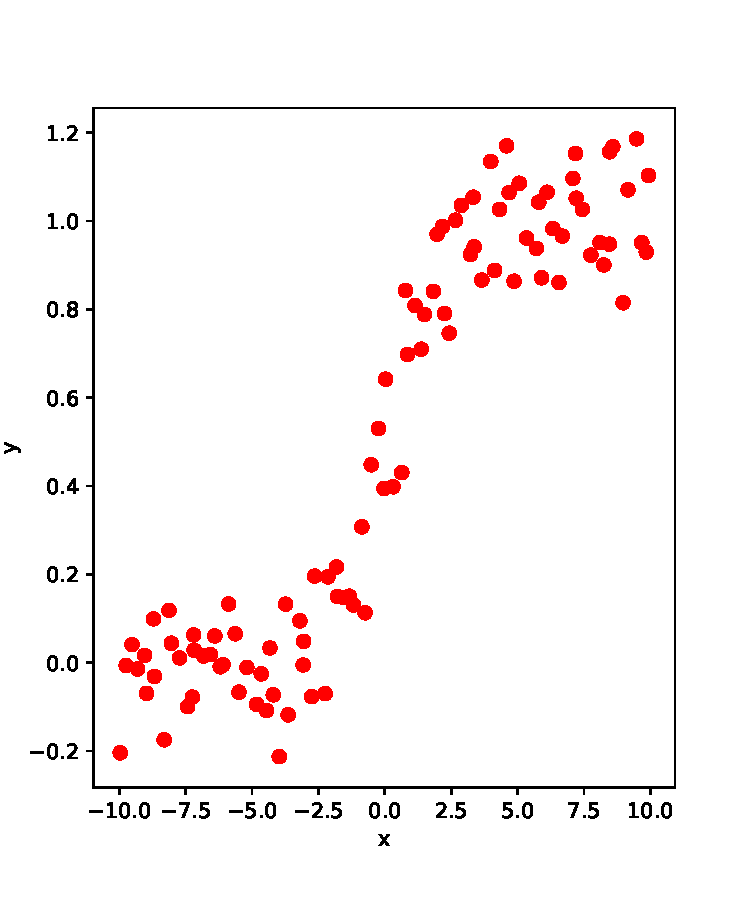
\includegraphics[width=\textwidth]{LSEx1Data.pdf}}
\end{columns}
\end{frame}

\begin{frame}[allowframebreaks=0.8]{Introductory Example -- Straight line}
\begin{columns}
\column{0.6\textwidth}
\begin{itemize}
\item Each pair of $a$ and $b$ represent one line.
\item Which line of the three would best describe the data set? 
Or some other line?
\end{itemize}
\column{0.45\textwidth}
\centerline{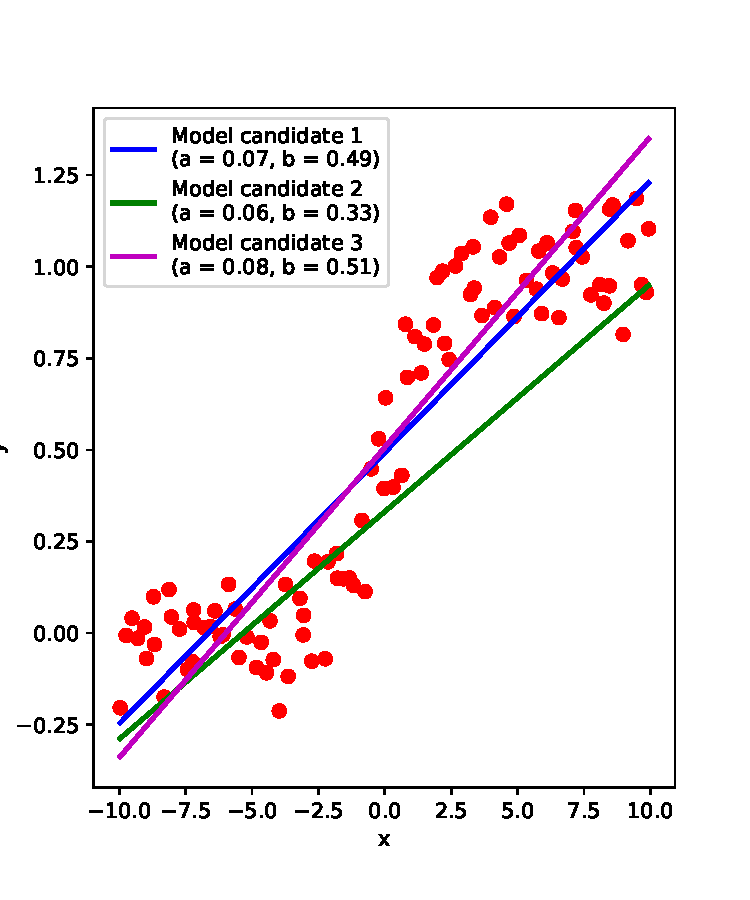
\includegraphics[width=\textwidth]{LSEx1.pdf}}
\end{columns}
\end{frame}

\begin{frame}[allowframebreaks=0.8]{Introductory Example -- Straight line}
\begin{itemize}
\item It can be shown that the best solution (in the \emph{maximum likelihood} sense; 
to be defined later) is given by
\begin{eqnarray*}
\hat{a} &=& - \frac{6}{N(N+1)}\sum_{n=0}^{N-1}y(n) + \frac{12}{N(N^2-1)}\sum_{n=0}^{N-1}x(n)y(n)\\
\hat{b} &=& \frac{2(2N-1)}{N(N+1)}\sum_{n=0}^{N-1}y(n) - \frac{6}{N(N+1)}\sum_{n=0}^{N-1}x(n)y(n).
\label{eq:optLinModel}
\end{eqnarray*}
\item Or, as we will later learn, in an easy matrix form: 
\[
\hat{\thb} = 
\begin{pmatrix}\hat{a}\\ \hat{b}\end{pmatrix}
= (\X^T\X)^{-1}\X^T\y
\]
\end{itemize}
\end{frame}

\begin{frame}[allowframebreaks=0.8]{Introductory Example -- Straight line}
\begin{columns}
\column{0.6\textwidth}
\begin{itemize}
\item In this case, $\hat{a} = 0.07401$ and $\hat{b} = 0.49319$,
which produces the line shown on the right.
\item The line also minimizes the squared distances (green dashed lines) 
between the model (blue line) and the data (red circles).
\end{itemize}
\column{0.45\textwidth}
\centerline{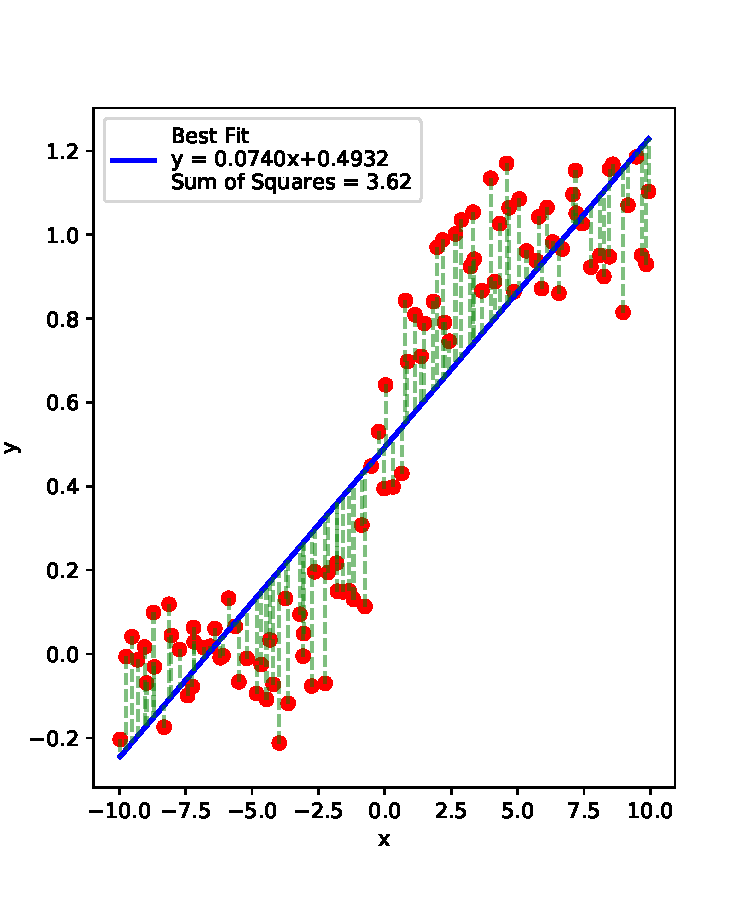
\includegraphics[width=\textwidth]{LSEx1Solution.pdf}}
\end{columns}
\end{frame}

\newcommand{\imagewidth}{0.6\textwidth}
\begin{frame}[allowframebreaks=0.8]{Introductory Example 2 -- Sinusoid}
 \begin{itemize}
\item Consider transmitting the sinusoid below.
\centerline{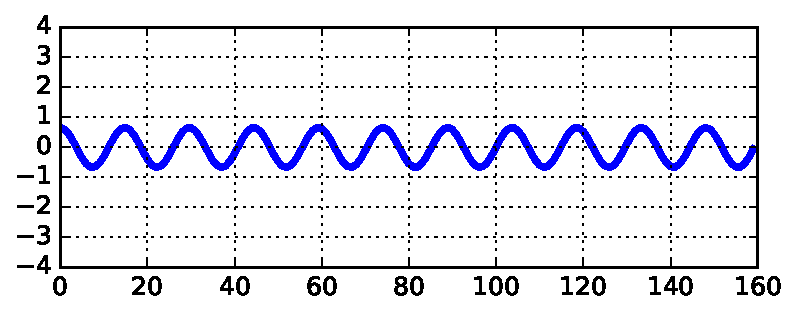
\includegraphics[width=\imagewidth]{MLSinusoidOrig.pdf}}
\item When the data is received, it is corrupted by noise
 and the received samples look like below.
\centerline{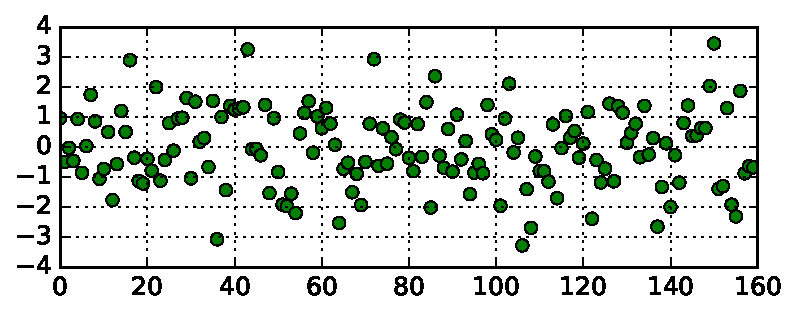
\includegraphics[width=\imagewidth]{MLSinusoidNoisy.pdf}} 
\item Can we recover the parameters of the sinusoid?
\end{itemize}
\end{frame}

\begin{frame}[allowframebreaks=0.8]{Introductory Example 2 -- Sinusoid}
 \begin{itemize}
\item In this case, the problem is to find good values for $A$,~%
$f_0$~and~$\phi$ in the following model:
\[
x[n] = A\cos(2\pi f_0 n + \phi) + w[n],
\]
with $w[n]\sim {\cal N}(0,\sigma^2)$.

\item It can be shown that the \emph{maximum likelihood estimator; MLE}
for parameters $A$, $f_0$ and $\phi$ are given by
\begin{eqnarray*}
\hat{f}_0 &=& \text{value of } f \text{ that maximizes } \left|\sum_{n=0}^{N-1} x(n)e^{-2\pi i f n}\right|,\\
\hat{A} &=& \frac2N \left|\sum_{n=0}^{N-1} x(n)e^{-2\pi i \hat{f}_0 n}\right| \\
\hat{\phi} &=& \arctan \frac{-\sum_{n=0}^{N-1} x(n)\sin(2\pi \hat{f}_0 n)}{\sum_{n=0}^{N-1} x(n)\cos(2\pi \hat{f}_0 n)}.
\end{eqnarray*}

\item It turns out that the sinusoidal parameter estimation is very
successful:
\centerline{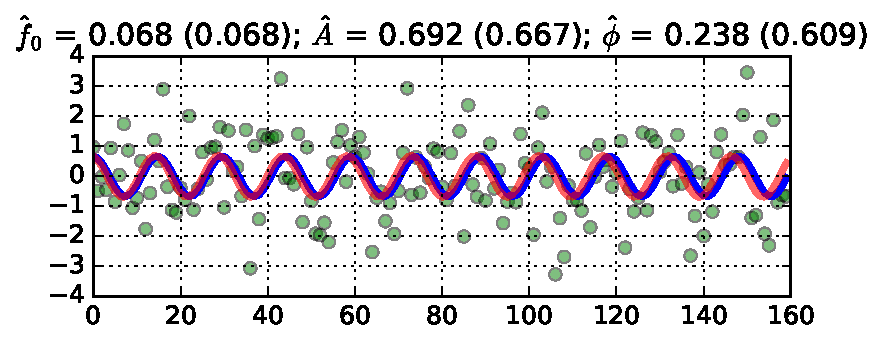
\includegraphics[width=\imagewidth]{MLSinusoid.pdf}}
\item The blue curve is the original sinusoid, and the red curve is the one estimated
from the green circles.
\item The estimates are shown in the figure (true values in parentheses).
\end{itemize}
\end{frame}

\begin{frame}{Introductory Example 2 -- Sinusoid}
 \begin{itemize}
\item However, the results are different for each \emph{realization} of the noise $w[n]$.
\end{itemize}
\begin{center}
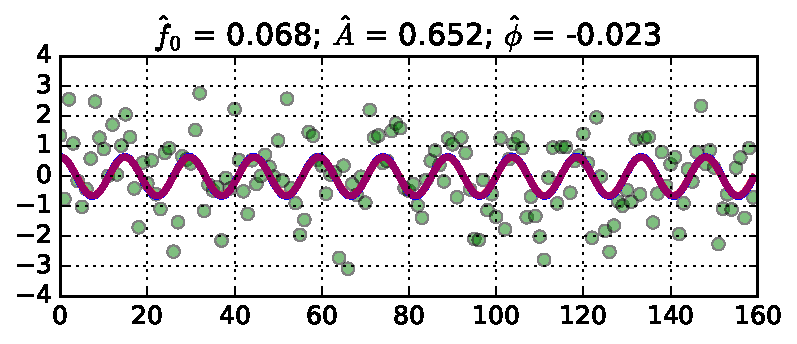
\includegraphics[width=0.47\textwidth]{MLSinusoid1.pdf}\quad
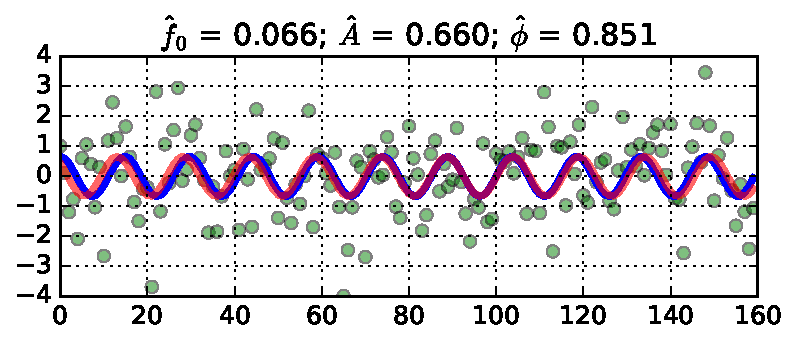
\includegraphics[width=0.47\textwidth]{MLSinusoid2.pdf}\\
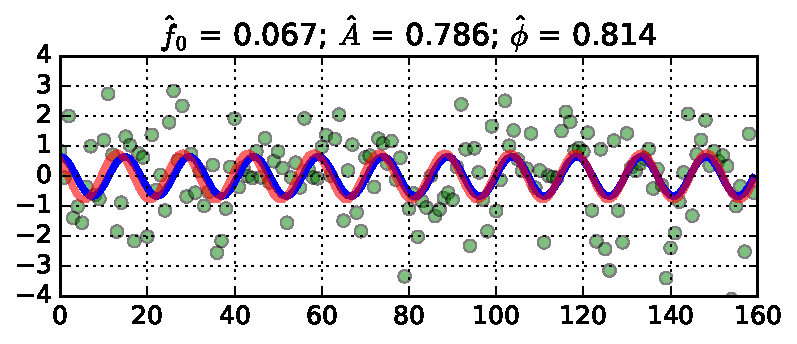
\includegraphics[width=0.47\textwidth]{MLSinusoid3.pdf}\quad
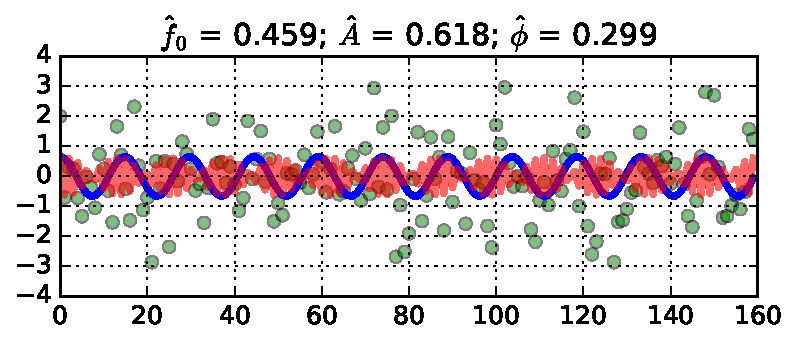
\includegraphics[width=0.47\textwidth]{MLSinusoid4.pdf}
\end{center}
\end{frame}

\begin{frame}[allowframebreaks=0.8]{Introductory Example 2 -- Sinusoid}
 \begin{itemize}


\item Thus, we're not very interested in an individual case, but rather on the distributions of estimates
 \begin{itemize}
 \item What are the expectations: $E[\hat{f_0}]$, $E[\hat{\phi}]$ and $E[\hat{A}]$?
 \item What are their respective variances?
 \item Could there be a better formula that would yield smaller variance?
 \item If yes, how to discover the better estimators?
\end{itemize}
\end{itemize}
\end{frame}


\begin{frame}
\vspace*{2cm}
\centerline{\Large LEAST SQUARES}
\end{frame}


%\begin{frame}[allowframebreaks=0.8]
 %{Least Squares}
 %\begin{itemize}
%\item First, we'll consider a class of estimators that in many cases have no optimality 
%properties associated with them, but are still applicable in a number of problems
%due to their ease of use.
%\item The \emph{Least Squares} approach originates from 1795, when Gauss
%invented the method (at the time he was only 18 years old)\footnote[frame]{\tiny Compare the date
%with maximum likelihood from 1912.\vspace*{0.4cm}}
%\item However, the method was properly formalized into its current form and published in 1806 by Legendre.
%\end{itemize}
%\end{frame}
%\begin{frame}[allowframebreaks=0.8]
 %{Least Squares}
%\begin{columns}
%\column{0.6\textwidth}
 %\begin{itemize}
%\item The method became widely known as Gauss was the only one able to describe
%the orbit of \emph{Ceres}, a minor planet in the asteroid belt between 
%Mars and Jupiter that was discovered in 1801.
  %\item In the least squares approach (LS) we attempt to minimize the
  %squared difference between the given data $x[n]$ and the assumed
  %signal model\footnote[frame]{\tiny In Gauss' case, the goal was to minimize
%the squared difference between the measurements of the location of Ceres and
%a family of functions describing the orbit.\vspace*{0.4cm}}.
%\item Note, that there is no assumption about the noise PDF.
%\end{itemize}
%\column{0.4\textwidth}
%\centerline{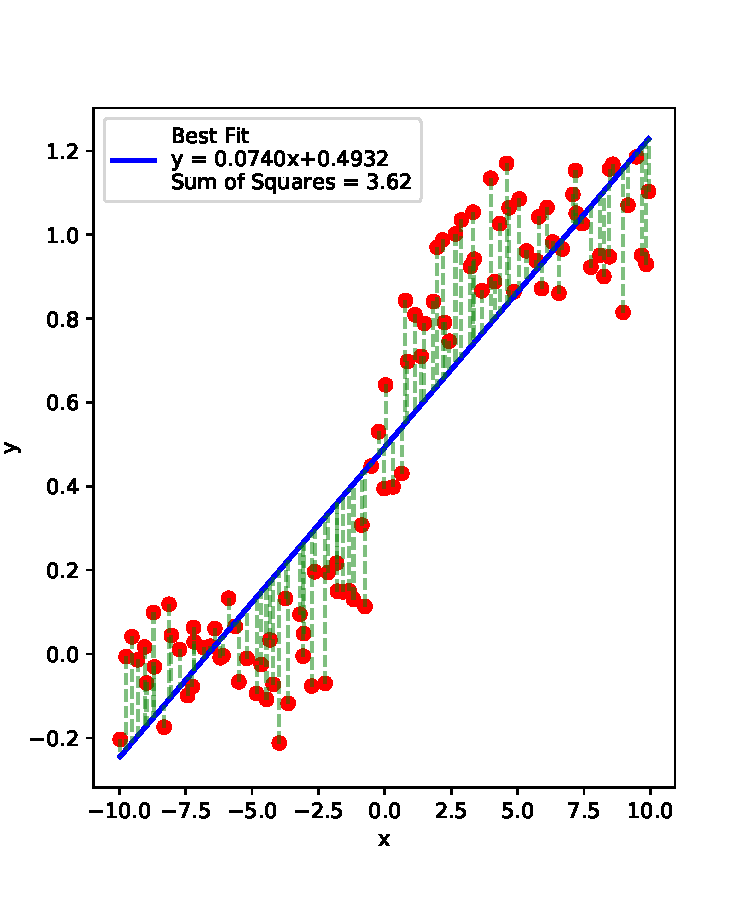
\includegraphics[width=\textwidth]{LSEx1Solution.pdf}}
%\end{columns}
%\end{frame}
%
%\begin{frame}[allowframebreaks=0.8]
 %{Least Squares}
 %\begin{itemize}
%\item The LS estimate $\hat{\theta}_{\text{LS}}$ is the value of $\theta$
%that minimizes the LS error criterion:
%\[
 %J(\theta) = \su (y[n]-s[n;\theta])^2.
%\]
%\item In the line fit case, $\thb = [a, b]^T$ and the LS criterion is
%\[
 %J(\thb) = \su (y[n]-s[n;\thb])^2 = \su (y[n]-(ax[n]+b))^2.
%\]
%\end{itemize}
%\end{frame}

\begin{frame}[allowframebreaks=0.8]
 {Least Squares}
 \begin{itemize}

\item The general solution for linear case is easy to remember.
\item Consider the line fitting case:
\(
y[n] = ax[n] + b + w[n].
\)
\item This can be written in matrix form as follows:
\[
\underbrace{\begin{pmatrix}
y[0]\\y[1]\\ \vdots\\y[N-1]
\end{pmatrix}}_{\y}
 = 
\underbrace{
\begin{pmatrix}
x[0] & 1\\
x[1] & 1\\
x[2] & 1\\
\vdots & \vdots\\
x[N-1] & 1
\end{pmatrix}}_{\X}
\underbrace{
\begin{pmatrix}a\\b\end{pmatrix}}_{\thb}
 + \boldsymbol{w}.
\]
\end{itemize}
\end{frame}


\begin{frame}[allowframebreaks=0.8]
 {Least Squares}
 \begin{itemize}
\item Now the model is written compactly as
\[
\y = \X\thb + \w
\]

\item Solution: The value of $\thb$ minimizing the error $\w^T\w$ is given by:
\[
\hat{\thb}_{LS} = \left(\X^T\X\right)^{-1}\X^T\y.
\]
\item See sample Python code here:
\url{https://github.com/mahehu/SGN-41007/blob/master/code/Least_Squares.ipynb}

\end{itemize}

\end{frame}

\begin{frame}
[allowframebreaks=0.8]
{LS Example with two variables}
\begin{columns}[onlytextwidth]
\column{0.63\textwidth}
\begin{itemize}
\item Consider an example, where microscope images have an uneven illumination.
\item The illumination pattern appears to have the highest brightness at the center.
\item Let's try to fit a paraboloid to remove the effect:
\[
z(x,y) = c_1 x^2 + c_2 y^2 + c_3xy + c_4x + c_5y + c_6,
\]
with $z(x,y)$ the brightness at pixel $(x,y)$.
\end{itemize}

\column{0.37\textwidth}
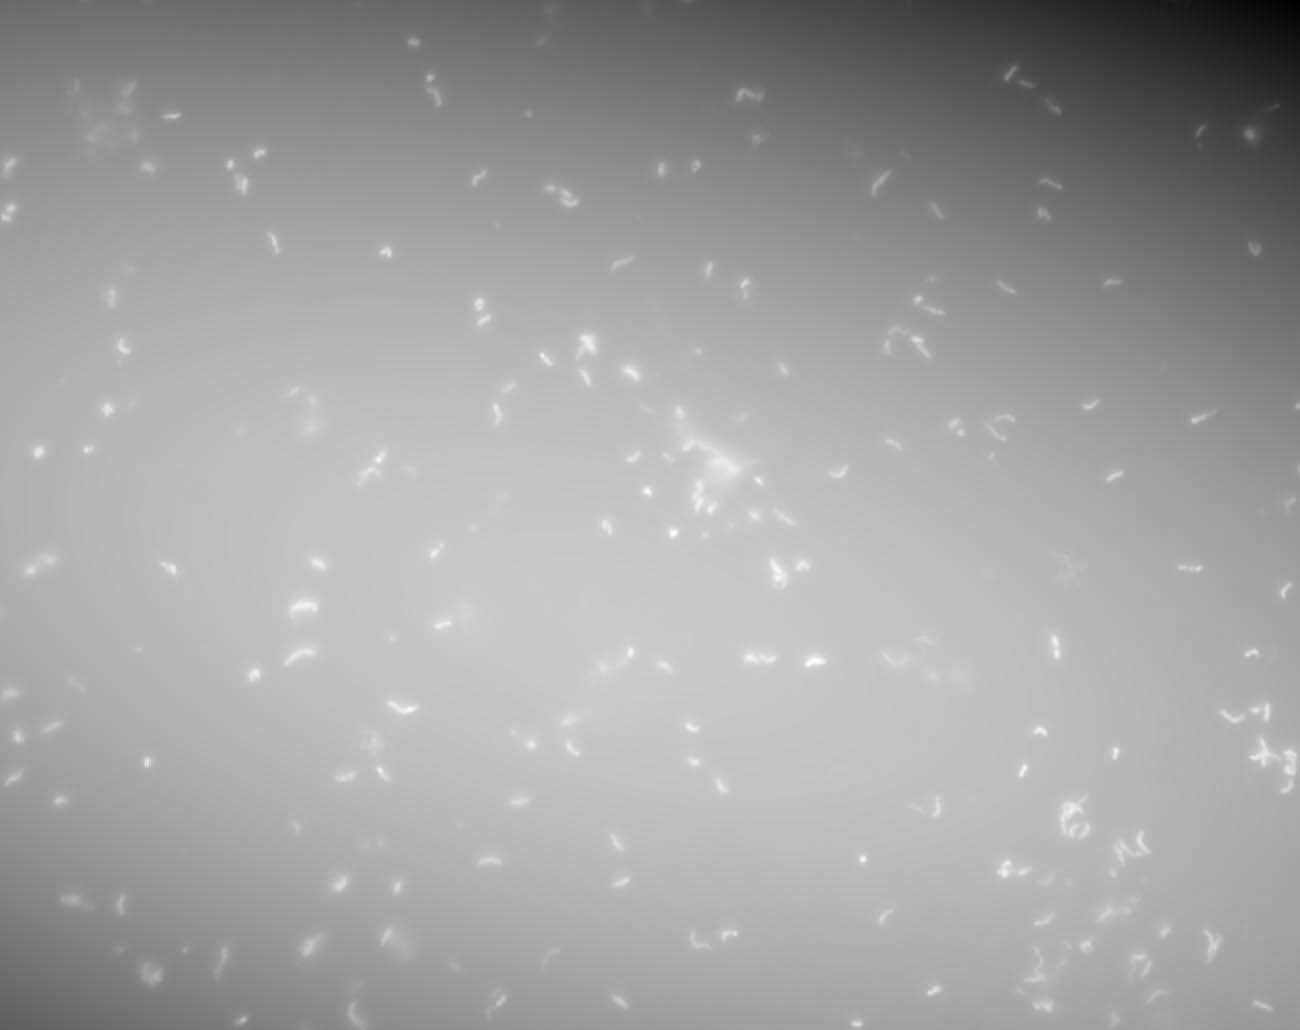
\includegraphics[width=\textwidth]{unevenIllumination}
\end{columns}

\end{frame}

\begin{frame}
[allowframebreaks=0.8]
{LS Example with two variables}
\begin{itemize}

\item In matrix form, the model looks like the following:
\begin{equation}
\underbrace{
\begin{pmatrix}
z_1\\z_2\\ \vdots\\ z_N
\end{pmatrix}}_{\bf z}
 = 
\underbrace{\begin{pmatrix}
x_1^2 & y_1^2 & x_1y_1 & x_1 & y_1 & 1\\
x_2^2 & y_2^2 & x_2y_2 & x_2 & y_2 & 1\\
\vdots&\vdots&\vdots&\vdots&\vdots&\vdots\\
x_N^2 & y_N^2 & x_Ny_N & x_N & y_N & 1
\end{pmatrix}}_{\bf H} \cdot 
\underbrace{\begin{pmatrix}
c_1\\c_2\\c_3\\c_4\\c_5\\c_6
\end{pmatrix}}_{\bf c} + \boldsymbol{\epsilon},
\label{eq:microscope}
\end{equation}
with $z_k$ the grayscale value at $k$'th pixel $(x_k, y_k)$. 
\item As a result we get the LS fit by $\hat{\mathbf{c}} = \left(\HH^T\HH\right)^{-1}\HH^T\z,$
\[
\hat{\mathbf{c}} = (-0.000080, -0.000288, \allowbreak 0.000123, \allowbreak 0.022064, \allowbreak
0.284020, 106.538687)
\]
\item Or, in other words
\begin{align*}
z(x,y) = &-0.000080x^2 -0.000288y^2 \\
       &+0.000123xy +0.022064x \\
			 &+0.284020y +106.538687.
\end{align*}

\end{itemize}

\end{frame}


\begin{frame}
[allowframebreaks=0.8]
{LS Example with two variables}
\begin{itemize}
\item Finally, we remove the illumination component by subtraction.
\end{itemize}

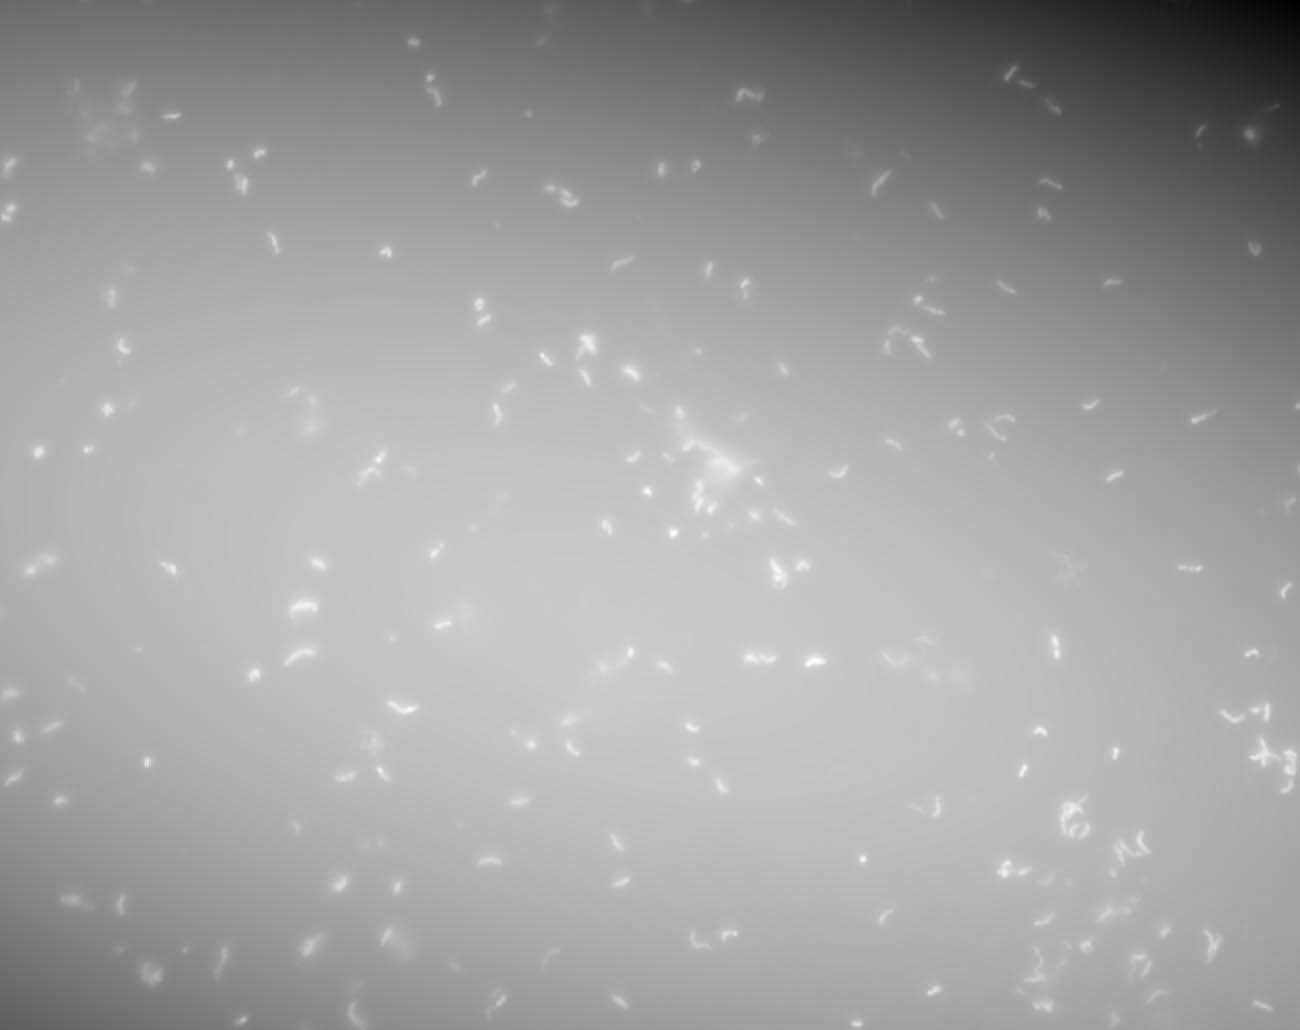
\includegraphics[width=0.3\textwidth]{unevenIllumination}
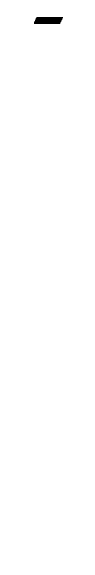
\includegraphics[height=2cm]{miinus}

\includegraphics[width=0.3\textwidth]{illuminationFit}
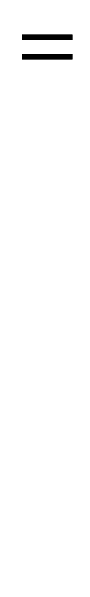
\includegraphics[height=2.1cm]{yhtasuuruus}
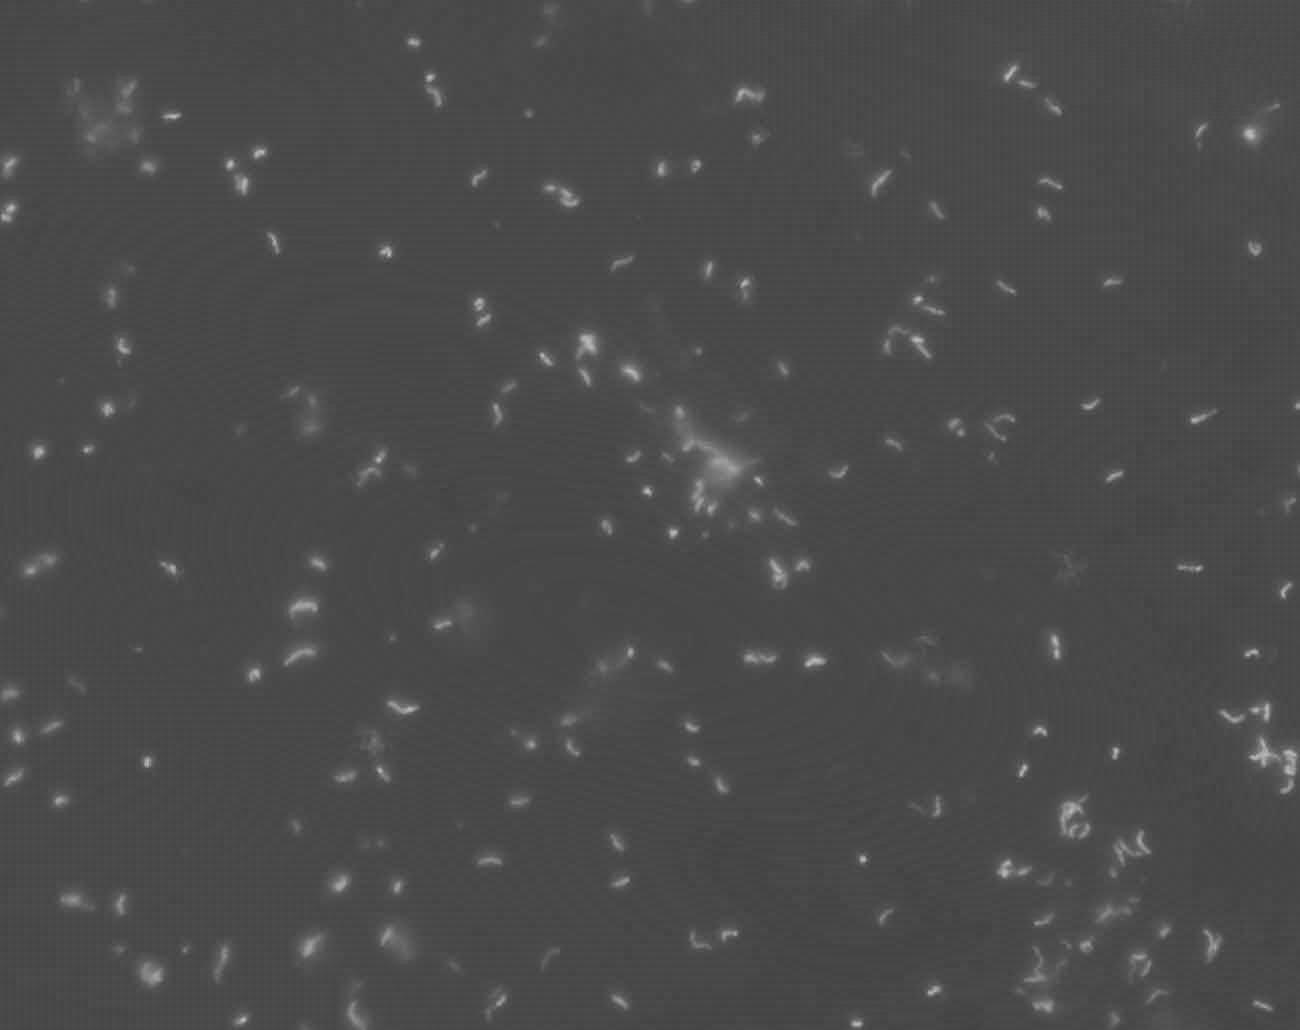
\includegraphics[width=0.3\textwidth]{LSResidual}


\end{frame}

%
%\begin{frame}
%\vspace*{2cm}
%\centerline{\Large ESTIMATOR VARIANCE}
%\end{frame}
%
%\begin{frame}[allowframebreaks=0.8]
%{Example of the Variance of an Estimator}
%\begin{itemize}
%\item Consider the estimation of the mean of the following measurement data:
%\centerline{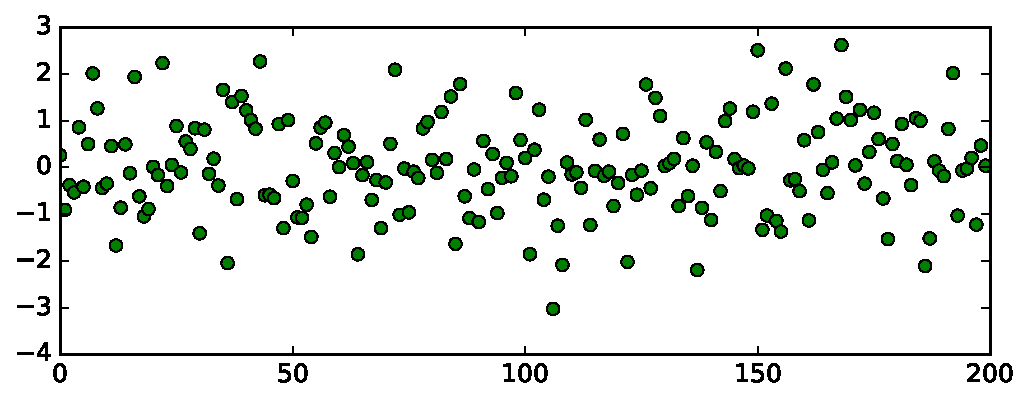
\includegraphics[width=0.7\textwidth]{GaussianRV.pdf}}
%\item Now we're searching for the estimator $\hat{A}$ in the model
%\[
%x[n] = A + w[n],
%\]
%with $w[n]\sim {\cal N}(0,\sigma^2)$ where $\sigma^2$ is also unknown.
%\item A natural estimator of $A$ is the sample mean:
%\[
%\hat{A} = \frac1N\sum_{n=0}^{N-1}x[n].
%\]
%\item Alternatively, one might propose to use only the first sample
%as such:
%\[
%\check{A} = x[0].
%\]
%\item How to justify that the first one is better?
%\end{itemize}
%\end{frame}
%
%\begin{frame}{Example of the Variance of an Estimator}
%\begin{columns}[onlytextwidth]
%\column{0.5\textwidth}
%\begin{itemize}
%\item Method 1: estimate variances \textbf{empirically}.
%\item Histograms of the estimates over 1000 data realizations are shown on the right.
%\item In other words, we synthesized 1000 versions of the data with the same
%statistics.
%\item Each synthetic sample produces one estimate of the mean for both estimators.
%\item Code available at \url{https://github.com/mahehu/SGN-41007/blob/master/code/Two_Estimators.ipynb}
%\begin{center}
%\end{center}
%\end{itemize}
%\column{0.55\textwidth}
%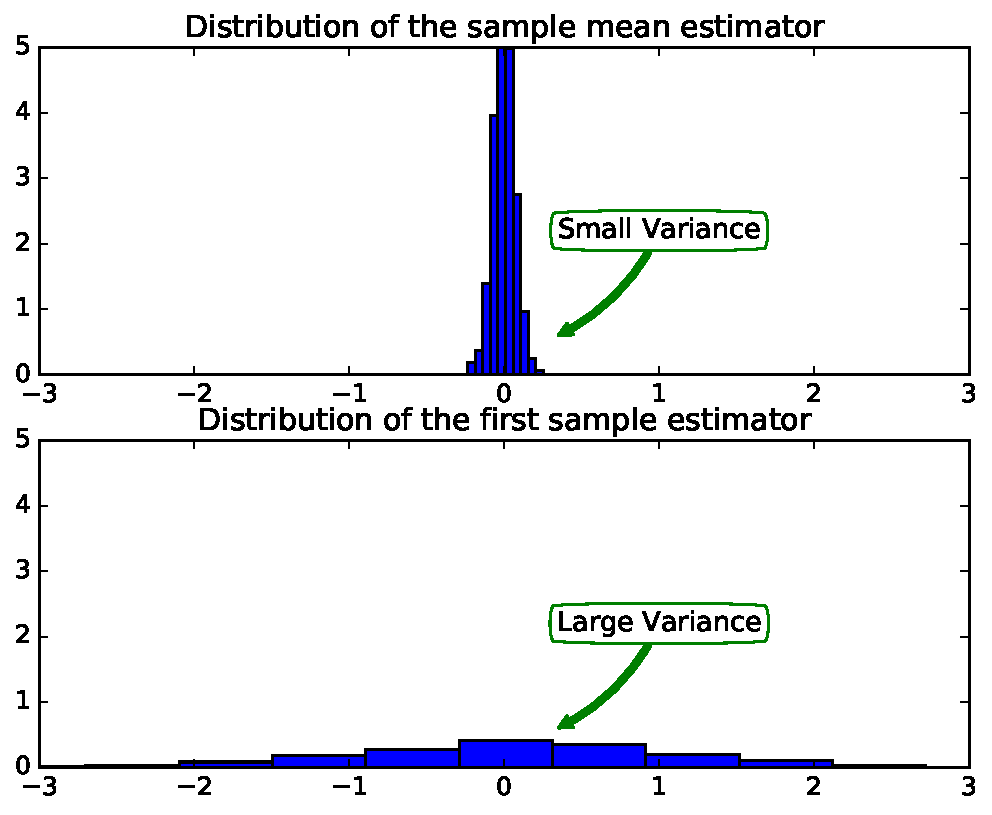
\includegraphics[width=\textwidth]{2Estimators.pdf}
%\end{columns}
%\end{frame}
%
%
%
%\begin{frame}{Example of the Variance of an Estimator}
%\begin{itemize}
%\item Method 2: estimate variances \textbf{analytically}.
%\item Namely, it is easy to compute variances in a closed form:
%\begin{alignat*}{2}
%\textbf{Estimator 1: } & \var(\hat{A}) &&= \var\left(\frac1N\sum_{n=0}^{N-1}x[n]\right)\\
%& && = \frac1{N^2}\sum_{n=0}^{N-1}\var(x[n])\\
%& && = \frac1{N^2}N\sigma^2 =\frac{\sigma^2}{N}. \qquad \Leftarrow \fbox{\text{good estimator}}\\
%\textbf{Estimator 2: } & \var(\check{A}) && = \var(x[0]) = \sigma^2. \qquad \Leftarrow \fbox{\text{bad estimator}}
%\end{alignat*}
%\end{itemize}
%\end{frame}
%%
%%\begin{frame}{Example of the Variance of an Estimator}
%%\begin{itemize}
%%\item Compared to the "First sample estimator"\ $\check{A} = x[0]$, the estimator variance of $\hat{A}$ is one $N$'th.
%%\item The analytical approach is clearly the desired one whenever possible:
%%\begin{itemize}
%%\item Faster, more elegant and less prone to random effects.
%%\item Often also provides proof that there exists no estimator that would be more efficient.
%%\end{itemize}
%%\item Usually can be done for easy cases.
%%\item More complicated scenarios can only be studied empirically.
%%\end{itemize}
%%\end{frame}
%
%\begin{frame}{Estimator Design}
%\begin{itemize}
%\item There are a few well established approaches for estimator design:
%\begin{itemize}
%\item \textbf{Minimum Variance Unbiased Estimator (MVU):} Analytically discover the estimator
%that minimizes the output variance among all \emph{unbiased} estimators.
%\item \textbf{Maximum Likelihood Estimator (MLE):} Analytically discover the estimator
%that maximizes the likelihood of observing the measured data.
%\item Others: \textbf{Method of Moments (MoM)} and \textbf{Least Squares (LS)}.
%\end{itemize}
%\item Our emphasis will be on Maximum Likelihood, as it appears in the machine learning part as well.
%\item Note, that different methods often (not always) result in the same estimator.
%\item For example, the MVU, MLE, MoM and LS estimators for the mean parameter all end up at the
%same formula: $\hat{A} = \frac1N\sum x_n$.
%\end{itemize}
%\end{frame}
%
%\begin{frame}{Minimum Variance Unbiased Estimator}
%\begin{columns}
%\column{0.6\textwidth}
%\begin{itemize}
%\item Commonly the MVU estimator is considered optimal.
%\item However, finding the MVU estimator may be difficult. The MVUE may not even exist.
%\item We will not concentrate on this estimator design approach.
%Interested reader may consult, \emph{e.g.}, S. Kay: \emph{Fundamentals of Statistical Signal Processing: Volume 1}  (1993).
%\item For an overview, read Wikipedia articles on \emph{Minimum-variance unbiased estimator}
%and \emph{Lehmann--Scheff\'e theorem}.
%\end{itemize}
%\column{0.47\textwidth}
%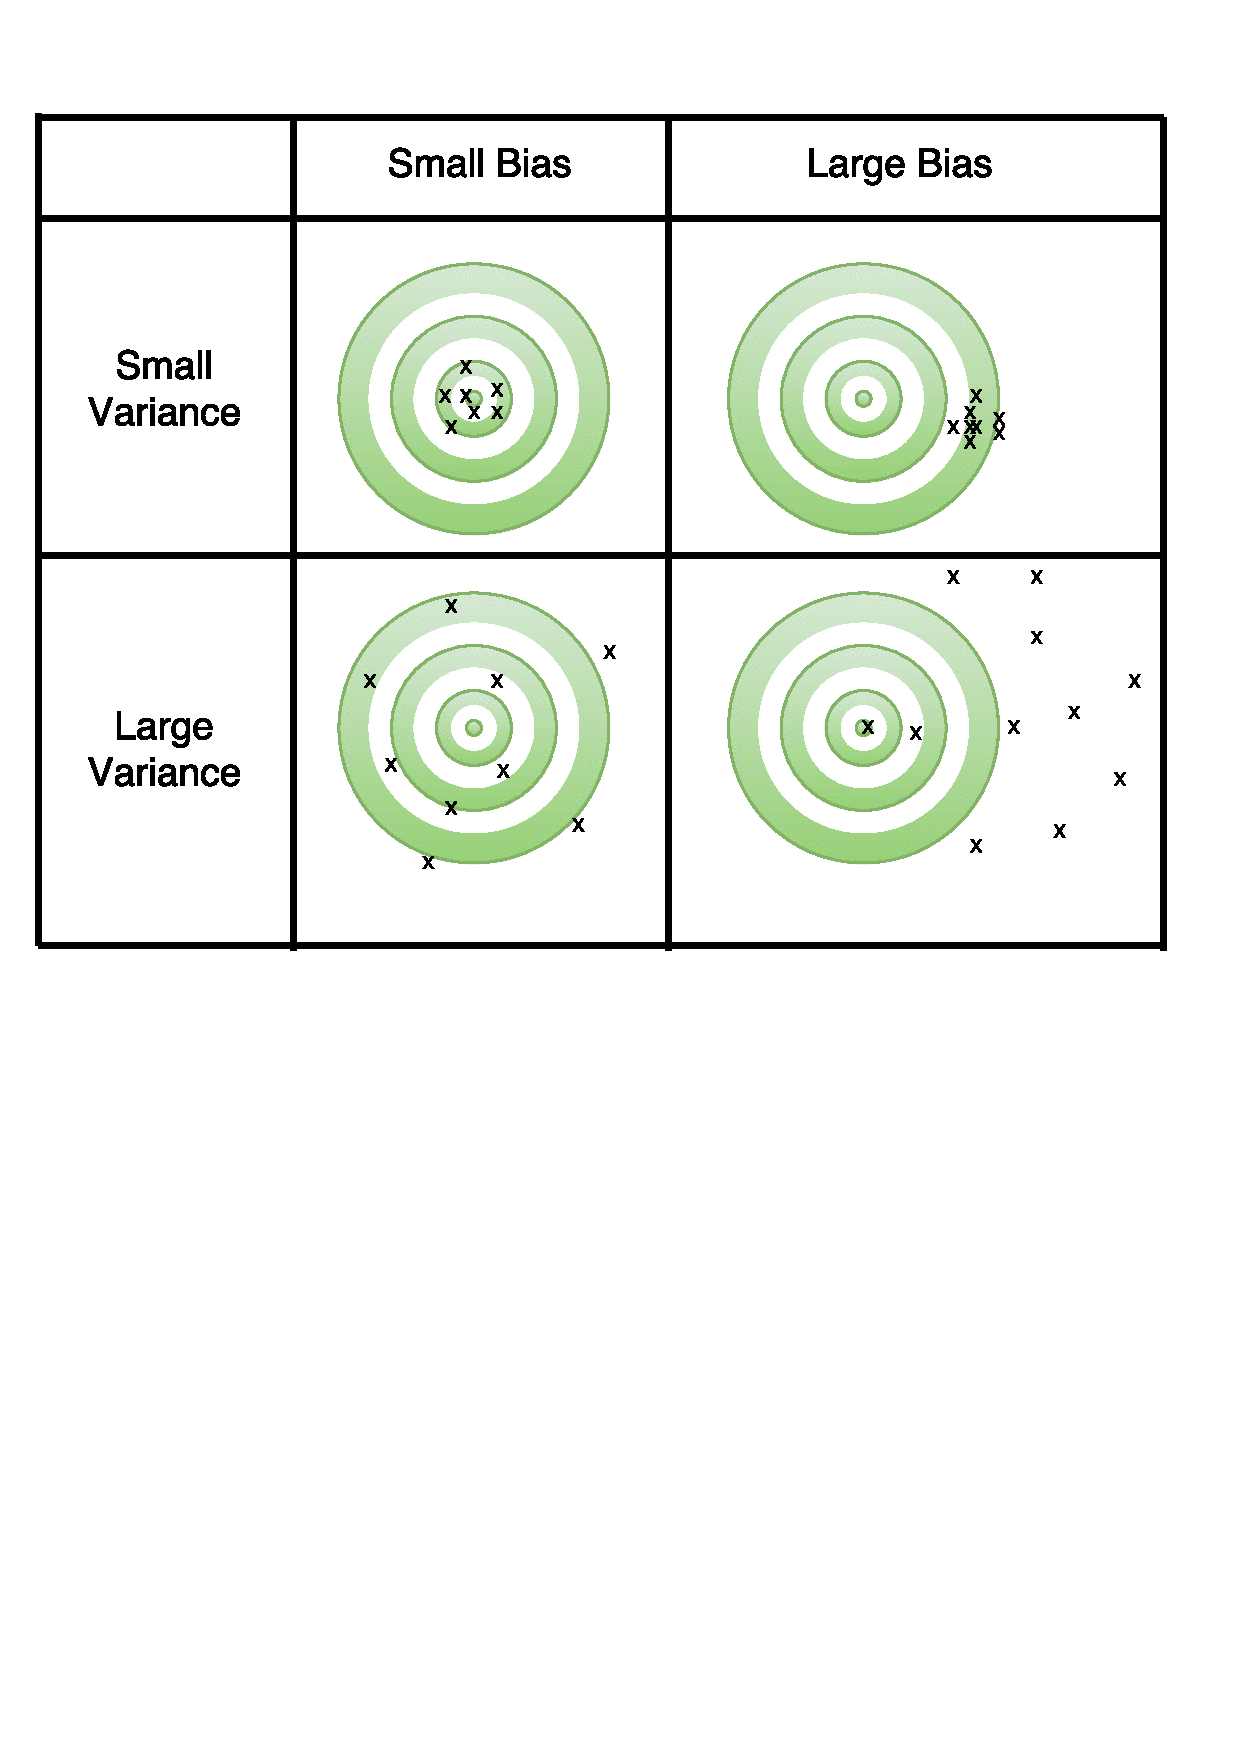
\includegraphics[width=\textwidth]{BiasVariance.pdf}
%\end{columns}
%\end{frame}


\begin{frame}
\vspace*{2cm}
\centerline{\Large MAXIMUM LIKELIHOOD}
\end{frame}


\begin{frame}[allowframebreaks=0.8]
{Maximum Likelihood Estimation}
\begin{itemize}
\item Maximum likelihood (MLE) is the most popular estimation approach
  due to its applicability in complicated estimation problems.
	\item Maximization of likelihood also appears often as the optimality criterion in machine learning.
\item The method was proposed by Fisher in 1922, though he published
  the basic principle already in 1912 as a third year undergraduate.
\item The basic principle is simple: find the parameter $\theta$ that
  is the most probable to have generated the data $\x$.
\item The MLE estimator may or may not be optimal in the minimum
  variance sense. It is not necessarily unbiased, either.
\end{itemize}
\end{frame}

\begin{frame}[allowframebreaks=0.8]{The Likelihood Function}
\begin{itemize}
\item Consider again the problem of estimating the mean level $A$ of noisy data.
\item Assume that the data originates from the following model:
\[
x[n] = A + w[n],
\]
where $w[n] \sim {\cal N}(0,\sigma^2)$: Constant plus Gaussian random noise with zero mean and variance $\sigma^2$.
\end{itemize}
\centerline{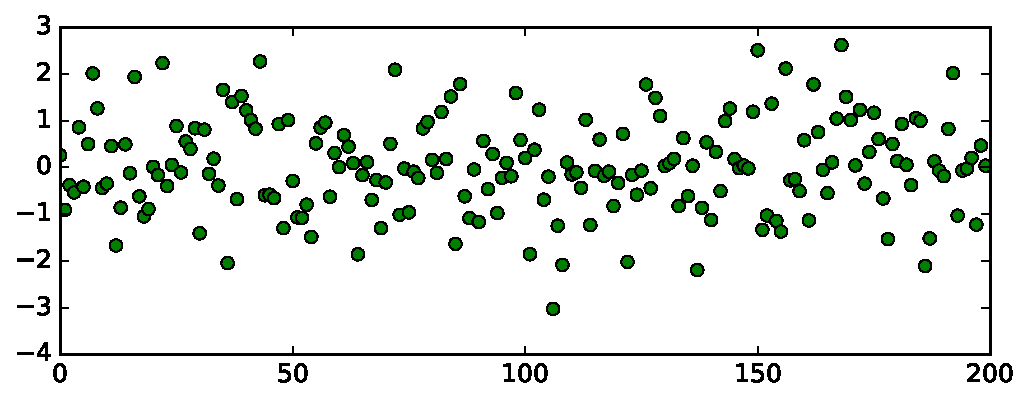
\includegraphics[width = 0.5\textwidth]{GaussianRV.pdf}}
\end{frame}

%\begin{frame}[allowframebreaks=0.8]{The Likelihood Function}
%\begin{itemize}
%\item For simplicity, consider the first sample estimator for estimating $A$.
%\item We assume normally distributed $w[n]$, \emph{i.e.,} the following  probability density function (PDF):
%\[
%p(w[n]) = \frac{1}{\sqrt{2\pi\sigma^2}}\exp\left[{-\frac{1}{2\sigma^2}(w[n])^2}\right]
%\]
%\item Since $x[n] = A + w[n]$, we can substitute $w[n] = x[n] - A$ above to describe the PDF of
%$x[n]$\footnote{We denote $p(x[n];A)$ to emphasize that $p$ depends on $A$.}:
%\[
%p(x[n]; A) = \frac{1}{\sqrt{2\pi\sigma^2}}\exp\left[{-\frac{1}{2\sigma^2}(x[n]-A)^2}\right]
%\]
%\end{itemize}
%\end{frame}
%
%\begin{frame}[allowframebreaks=0.8]{The Likelihood Function}
%\begin{itemize}
%\item Thus, our first sample estimator has the PDF
%\[
%p(x[0]; A) = \frac{1}{\sqrt{2\pi\sigma^2}}\exp\left[{-\frac{1}{2\sigma^2}(x[0]-A)^2}\right]
%\]
%\item Now, suppose we have observed $x[0]$, say $x[0] = 3$.
%\item Then some values of $A$ are more likely than others
%and we can derive the complete PDF of $A$ easily.
%\end{itemize}
%\end{frame}
%
%\begin{frame}[allowframebreaks=0.8]{The Likelihood Function}
%\begin{itemize}
%\item Actually, the PDF of $A$ has the same form as the PDF of $x[0]$:
%\[
%\text{pdf of } A = \frac{1}{\sqrt{2\pi\sigma^2}}\exp\left[{-\frac{1}{2\sigma^2}(3-A)^2}\right]
%\]
%\end{itemize}
%\centerline{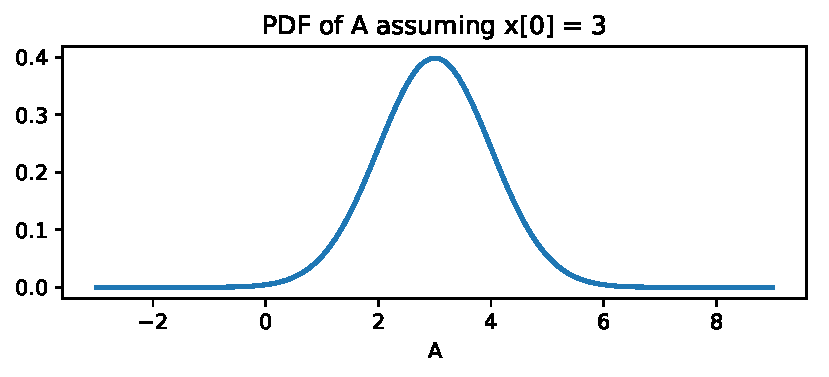
\includegraphics[width=0.4\textwidth]{PDF_A.pdf}}
%\begin{itemize}
%\item This function is called \emph{the likelihood function} of $A$, and its maximum
%the \emph{maximum likelihood estimate}.
%\end{itemize}
%\end{frame}

\begin{frame}[allowframebreaks=0.8]{The Likelihood Function}
\begin{itemize}
\item The key to maximum likelihood is the \emph{likelihood function}.
\item If the probability density function (PDF) of the data is viewed as a function of the unknown 
parameter (with fixed data), it is called likelihood function.
\item Often the likelihood function has an exponential form. Then it's usual to
take the natural logarithm to get rid of the exponential. Note that the maximum of
the new \emph{log-likelihood} function does not change.
\end{itemize}
\centerline{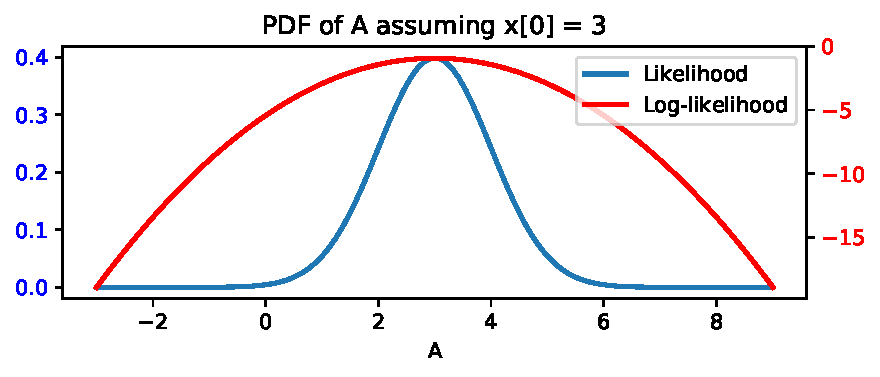
\includegraphics[width=0.5\textwidth]{PDF_A_LL.pdf}}
\end{frame}

\begin{frame}[allowframebreaks=0.8]
{MLE Example}

\begin{itemize}
\item In our case of estimating the mean of a signal:
\[
x[n] = A + w[n],\qquad n=0,1,\ldots, N-1,
\]
the likelihood function is easy to construct.
\item The noise samples $w[n]\sim {\cal N}(0,\sigma^2)$ are assumed independent, so the PDF
of the whole batch of samples $\x = (x[0],\ldots, x[N-1])$ is obtained by the product rule:
\[
p({\x};A) = \prod_{n = 0}^{N-1} p(x[n]; A) = \frac{1}{(2 \pi \sigma^2)^{\frac{N}{2}}} \exp\left[-
  \frac{1}{2\sigma^2} \sum_{n=0}^{N-1} (x[n]-A)^2\right]
\]
\item When we have observed the data $\x$, we can turn the problem
  around and consider \emph{what is the most likely parameter $A$ to have
  generated the data}.
\item Some authors emphasize this by turning the order around:
  $p(A;\x)$ or give the function a different name such as $L(A; \x)$
  or $\ell(A;\x)$.
\item So, consider $p(\x;A)$ as a function of $A$ and try to maximize
  it.
\end{itemize}
\end{frame}

\begin{frame}[allowframebreaks=0.8]
{MLE Example}

\begin{itemize}
\item  The picture below shows the likelihood function and the
  log-likelihood function for one possible realization of data.
\item The data consists of 50 points, with true $A=5$. 
\item The likelihood function gives the
  probability of observing these particular points with different
  values of $A$.
\end{itemize}
\centerline{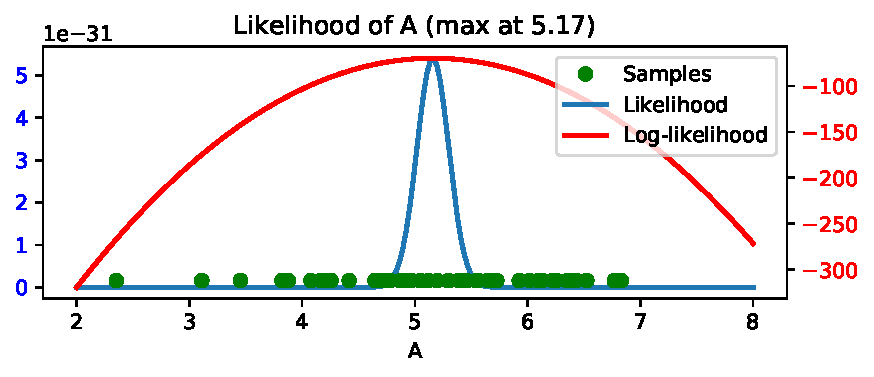
\includegraphics[width=0.5\textwidth]{PDF_A_LL_full.pdf}}
\end{frame}

\begin{frame}[fragile,allowframebreaks=0.8]
{MLE Example}
\begin{itemize}
\item Instead of finding the maximum from the plot, 
we wish to have a closed form solution.
\item Closed form is faster, more elegant, accurate and numerically more stable.
\item Just for the sake of an example, below is the code for the stupid version.
\end{itemize}
\begin{center}
\begin{minipage}{9cm}
\begin{lstlisting}
# The samples are in array called x0

x = np.linspace(2, 8, 200)
likelihood = []
log_likelihood = []

for A in x:
    likelihood.append(gaussian(x0, A, 1).prod())
    log_likelihood.append(gaussian_log(x0, A, 1).sum())

print ("Max likelihood is at %.2f" % (x[np.argmax(log_likelihood)]))
\end{lstlisting}
\end{minipage}
\end{center}
\end{frame}

\begin{frame}[fragile,allowframebreaks=0.8]
{MLE Example}
\begin{itemize}
{\small
\item Maximization of $p(\x;A)$ directly is nontrivial. Therefore,
  we take the logarithm, and maximize it instead:
\begin{eqnarray*}
p({\x};A) &=& \frac{1}{(2 \pi \sigma^2)^{\frac{N}{2}}} \exp\Big[-
  \frac{1}{2\sigma^2} \sum_{n=0}^{N-1} (x[n]-A)^2\Big]\\
\ln p(\x;A) &=& -\frac N2 \ln(2\pi\sigma^2)-
  \frac{1}{2\sigma^2} \sum_{n=0}^{N-1} (x[n]-A)^2
\end{eqnarray*}
\item The maximum is found via differentiation:
\[
\frac{\partial\ln p(\x;A) }{\partial A} = 
  \frac{1}{\sigma^2} \sum_{n=0}^{N-1} (x[n]-A)
\]
\item Setting this equal to zero gives
}
{\scriptsize
\begin{eqnarray*}
\frac{1}{\sigma^2} \sum_{n=0}^{N-1} (x[n]-A) &=& 0\\
\sum_{n=0}^{N-1} (x[n]-A) &=& 0\\
\sum_{n=0}^{N-1} x[n] - \sum_{n=0}^{N-1} A &=& 0\\
\sum_{n=0}^{N-1} x[n] - NA &=& 0\\
\sum_{n=0}^{N-1} x[n] &=& NA \\
A &=& \frac1N \sum_{n=0}^{N-1} x[n]
\end{eqnarray*}
}
\end{itemize}
\end{frame}

\begin{frame}[allowframebreaks=0.8]
{Conclusion}

\begin{itemize}
\item \textit{What did we actually do?}
\begin{itemize}
\item We proved that the \textbf{sample mean} is the maximum likelihood estimator for the \textbf{distribution mean}.
\end{itemize}

\item \textit{But I could have guessed this result from the beginning. What's the point?}
\begin{itemize}
\item We can do the same thing for cases where you can not guess.
\end{itemize}
\end{itemize}
\end{frame}

\begin{frame}[allowframebreaks=0.8]
{Example: Sinusoidal Parameter Estimation}

\begin{itemize}
\item Consider the model
\[
 x[n] = A\cos(2\pi f_0 n + \phi) + w[n]
\]
with $w[n]\sim {\cal N}(0,\sigma^2)$. It is possible to find the MLE for all three parameters:
$\thb = [A, f_0, \phi]^T$.
\item The PDF is given as
\[
 p(\x;\thb) = \frac{1}{(2\pi\sigma^2)^{\frac N2}} \exp \left[ -\frac{1}{2\sigma^2}\sum_{n=0}^{N-1}(\underbrace{x[n]-A\cos(2\pi f_0 n + \phi)}_{w[n]})^2 \right]
\]
\item Instead of proceeding directly through the log-likelihood function, we note that the above function
is maximized when
\[
J(A, f_0,\phi) = \sum_{n=0}^{N-1}(x[n]-A\cos(2\pi f_0 n + \phi))^2
\]
is minimized.
\item The minimum of this function can be found although it is a nontrivial task (about 10 slides). 
\item We skip the derivation, but for details, see Kay \emph{et al.} "Statistical Signal Processing: Estimation Theory," 1993.
\end{itemize}
\end{frame}
\begin{frame}{Sinusoidal Parameter Estimation}
\begin{itemize}
{\small
\item The MLE of frequency $f_0$ is obtained by maximizing the \textit{periodogram} over $f_0$:
\[
 \hat{f}_0 = \argmax_{f}\left|\sum_{n=0}^{N-1}x[n]\exp( -j 2\pi f n)\right|
\]
\item Once $\hat{f}_0$ is available, proceed by calculating the other parameters:
\begin{align*}
 \hat{A} &= \frac 2N \left|\sum_{n=0}^{N-1}x[n]\exp( -j 2\pi \hat{f}_0 n)\right|\\
\hat{\phi} &= \arctan \left(-\frac{\sum\limits_{n=0}^{N-1}x[n]\sin 2\pi \hat{f}_0 n}{\sum\limits_{n=0}^{N-1}x[n]\cos 2\pi \hat{f}_0 n}\right) 
\end{align*}
}
\end{itemize}
\end{frame}

\begin{frame}{Sinusoidal Parameter Estimation---Experiments}
\begin{columns}
\column{0.65\textwidth}
\begin{itemize}
\item Four example runs of the estimation algorithm are illustrated in the figures.
\item The algorithm was also tested for 10000 realizations of a sinusoid with
fixed $\thb$ and $N=160$, $\sigma^2=1.2$.
\item Note that the estimator is not unbiased.
\end{itemize}
\column{0.35\textwidth}
\centerline{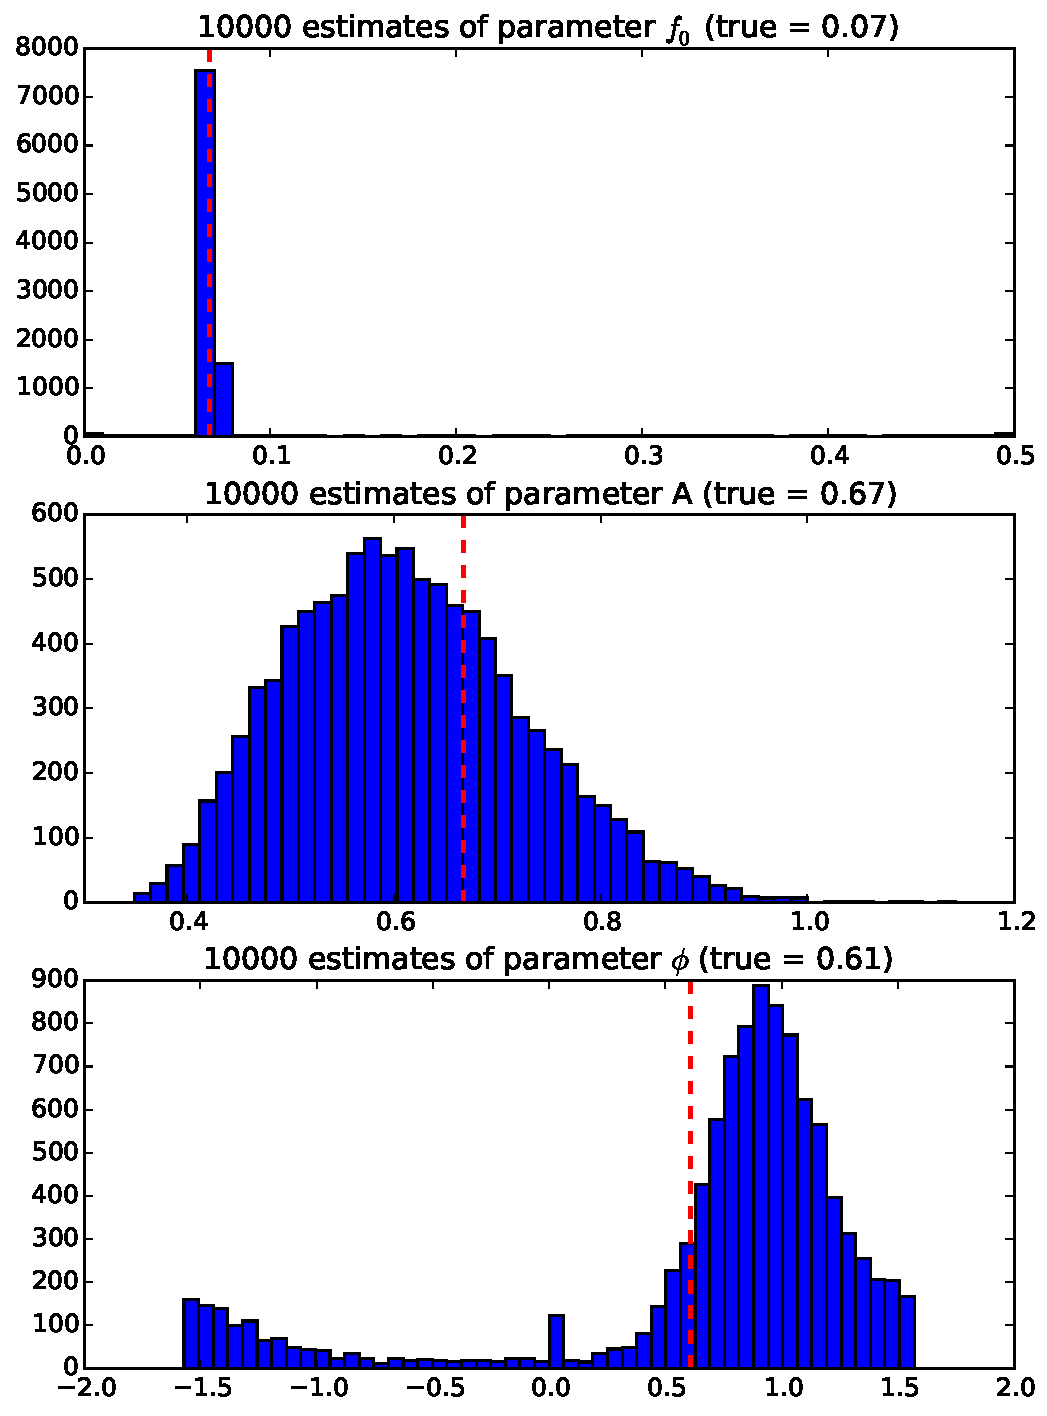
\includegraphics[width=\textwidth]{ML_sinusoid_batch.pdf}}
\end{columns}
\end{frame}



\begin{frame}{Estimation Theory---Summary}
\begin{itemize}
\item We have seen a brief overview of estimation theory with particular focus on Maximum Likelihood.
\item If your problem is simple enough to be modeled by an equation, the estimation theory is the answer.
\begin{itemize}
\item Estimating the frequency of a sinusoid is completely solved by classical theory.
\item Estimating the age of the person in picture can not possibly be modeled this simply and classical theory has no answer.
\end{itemize}
\item \textbf{Model based }estimation is the best answer when a model exists.
\item Machine learning can be understood as \textbf{a data driven approach}.
\end{itemize}
\end{frame}

\end{document}

